\documentclass[11pt]{article}
\usepackage[utf8]{inputenc}

%%% PAGE DIMENSIONS
\usepackage{geometry}
\geometry{a4paper}

\usepackage{graphicx}

%%% PACKAGES
\usepackage{booktabs}
\usepackage{paralist}
\usepackage{verbatim}
\usepackage{subfig}
\usepackage{chngcntr}
\usepackage{tikz}
\usepackage[colorlinks = true,
            linkcolor = black,
            urlcolor  = blue,
            citecolor = blue,
            anchorcolor = blue]{hyperref}
\usepackage[spanish]{cleveref}
\usepackage{placeins}
\usepackage{float}
\usepackage{listings}

%%% HEADERS & FOOTERS
\usepackage{fancyhdr}
\pagestyle{fancy}
\renewcommand{\headrulewidth}{0pt}
\lhead{}\chead{}\rhead{}
\lfoot{}\cfoot{\thepage}\rfoot{}

%%% SECTION TITLE APPEARANCE
\usepackage{sectsty}
\allsectionsfont{\sffamily\mdseries\upshape}

%%% ToC (table of contents) APPEARANCE
\usepackage[nottoc,notlof,notlot]{tocbibind} % Put the bibliography in the ToC
\usepackage[titles,subfigure]{tocloft} % Alter the style of the Table of Contents
\renewcommand{\cftsecfont}{\rmfamily\mdseries\upshape}
\renewcommand{\cftsecpagefont}{\rmfamily\mdseries\upshape} % No bold!


\graphicspath{ {images/} }

\counterwithin*{figure}{section}
\counterwithin*{figure}{subsection}
\counterwithin*{figure}{subsubsection}

\counterwithin*{table}{section}
\counterwithin*{table}{subsection}
\counterwithin*{table}{subsubsection}

\addtolength{\cftfignumwidth}{2em}

\renewcommand{\thefigure}{
  \ifnum\value{subsection}=0
    \thesection.\arabic{figure}
  \else
    \ifnum\value{subsubsection}=0
      \thesubsection.\arabic{figure}
    \else
      \thesubsubsection.\arabic{figure}
    \fi
  \fi
}

\renewcommand{\thetable}{
  \ifnum\value{subsection}=0
    \thesection.\arabic{table}
  \else
    \ifnum\value{subsubsection}=0
      \thesubsection.\arabic{table}
    \else
      \thesubsubsection.\arabic{table}
    \fi
  \fi
}

%%% END Article customizations

%%% The "real" document content comes below...

\title{\Large Seguridad en Redes\\Practica 4.2}
\author{David Antuña Rodríguez\\Javier Carrión García}
\date{}

\begin{document}
  \raggedright

  \maketitle
  \newpage

  \section{Configuración de HTTPS}
    \par
    La conexión tiene las siguientes propiedades.
    \begin{itemize}
      \item TLS versión 1.1
      \item Encriptación: AES\_128\_CBC
      \item Autenticación: SHA1
      \item Intercambio de clave: ECDHE\_RSA
    \end{itemize}

    \par
    El cliente y el servidor realizan el handshake típico, en el último paso
    el servidor le extiende un ticket de sesión al cliente.

    \begin{figure}[H]
      \centering
      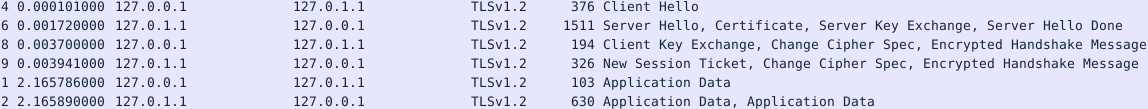
\includegraphics[width = \textwidth]{tls1}
      \caption{Acuerdo TLS}
    \end{figure}


    \par
    El handshake es idéntico al anterior salvo que en el saludo del servidor
    también ha enviado la clave.

    \begin{figure}[H]
      \centering
      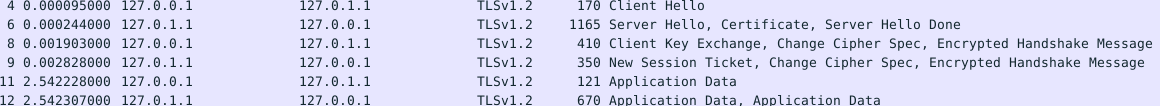
\includegraphics[width = \textwidth]{tls2}
      \caption{Acuerdo TLS con -cipher}
    \end{figure}

    \par
    El cliente envia el id de sesión en el saludo, primer mensaje, ahora tan
    solo se necesitan 3 mensajes para crear la conexión, se elimina el mensaje
    del servidor que envia el ticket de sesión.

    \begin{figure}[H]
      \centering
      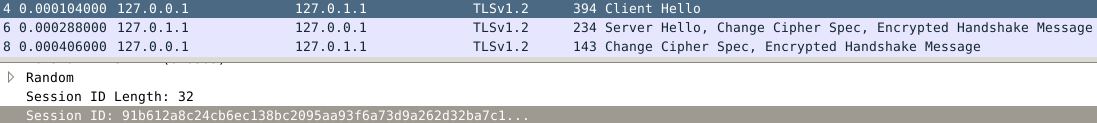
\includegraphics[width = \textwidth]{tls3}
      \caption{Acuerdo TLS de la sesión almacenada}
    \end{figure}


  \section{Autenticación del cliente mediante certificado}
    \par
    El handshake ocurre de forma similar pero tras el saludo del servidor el
    cliente envia su certificado en conjunto con lo que ya enviaba.

    \begin{figure}[H]
      \centering
      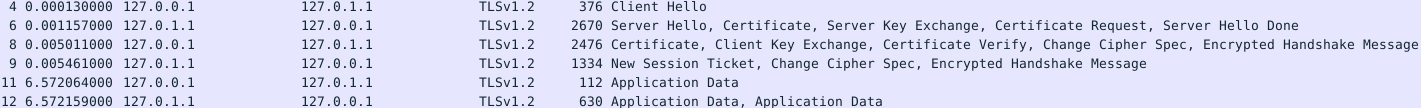
\includegraphics[width = \textwidth]{tls_client}
      \caption{Mensajes obtenidos en Wireshark}
    \end{figure}
\end{document}
